% Generated by LitigCharts.PublicationFigures. Captions and provenance are sidecars.
\documentclass[10pt,tikz,border=5pt]{standalone}
\usepackage{lmodern}
\usetikzlibrary{patterns,patterns.meta}
\begin{document}
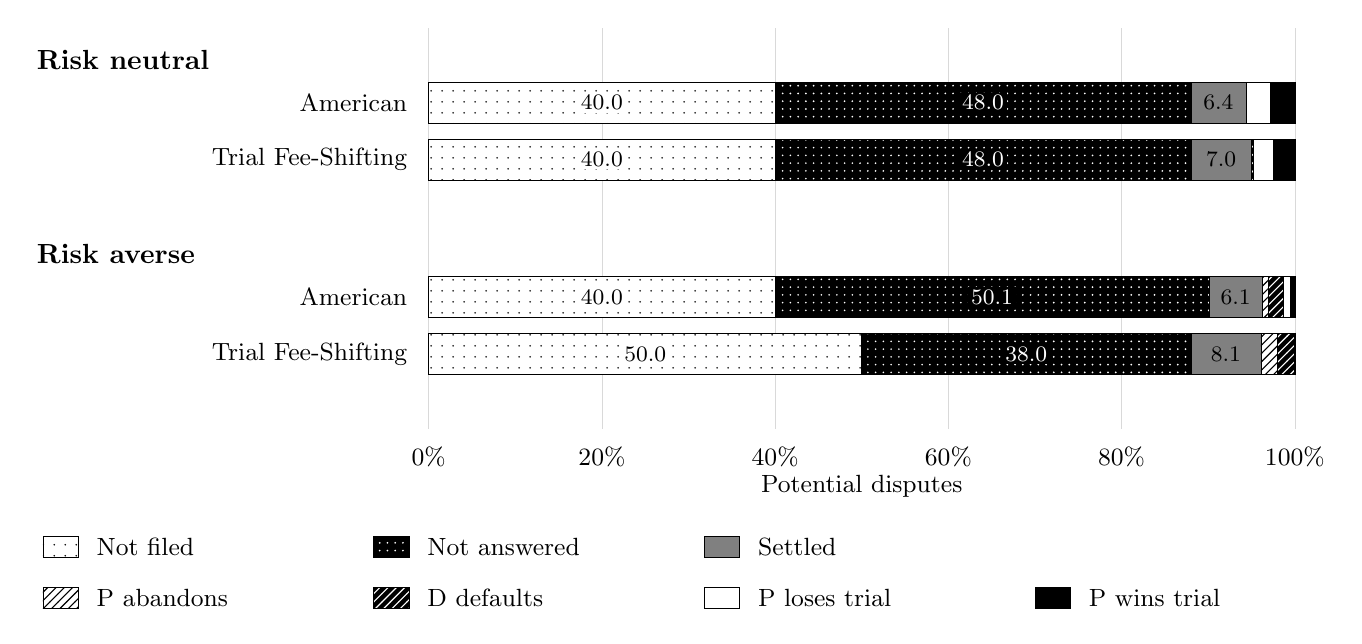
\begin{tikzpicture}[font=\small]\draw[black!15,line width=.2pt] (5.1,.65) -- (5.1,5.74);
\node[anchor=north] at (5.1,.55) {0\%};
\draw[black!15,line width=.2pt] (7.3,.65) -- (7.3,5.74);
\node[anchor=north] at (7.3,.55) {20\%};
\draw[black!15,line width=.2pt] (9.5,.65) -- (9.5,5.74);
\node[anchor=north] at (9.5,.55) {40\%};
\draw[black!15,line width=.2pt] (11.7,.65) -- (11.7,5.74);
\node[anchor=north] at (11.7,.55) {60\%};
\draw[black!15,line width=.2pt] (13.9,.65) -- (13.9,5.74);
\node[anchor=north] at (13.9,.55) {80\%};
\draw[black!15,line width=.2pt] (16.1,.65) -- (16.1,5.74);
\node[anchor=north] at (16.1,.55) {100\%};
\node[anchor=west,font=\bfseries] at (0,5.34) {\mbox{Risk} \mbox{neutral}};
\node[anchor=east] at (4.95,4.79) {American};
\path[preaction={fill=white,draw=none},pattern={Dots[distance=4pt,radius=.35pt]},pattern color=black,draw=black,line width=.25pt] (5.1,4.53) rectangle (9.49879,5.05);
\node[text=black,fill=white,font=\footnotesize,inner sep=1pt] at (7.299395,4.79) {40.0};
\path[preaction={fill=black,draw=none},pattern={Dots[distance=2.8pt,radius=.35pt]},pattern color=white,draw=black,line width=.25pt] (9.49879,4.53) rectangle (14.77923,5.05);
\node[text=white,fill=black,font=\footnotesize,inner sep=1pt] at (12.13901,4.79) {48.0};
\path[fill=black!50,draw=black,line width=.25pt] (14.77923,4.53) rectangle (15.479244,5.05);
\node[text=black,fill=none,font=\footnotesize,inner sep=1pt] at (15.129237,4.79) {6.4};
\path[fill=white,draw=black,line width=.25pt] (15.479244,4.53) rectangle (15.789621,5.05);
\path[fill=black,draw=black,line width=.25pt] (15.789621,4.53) rectangle (16.1,5.05);
\node[anchor=east] at (4.95,4.07) {Trial Fee-Shifting};
\path[preaction={fill=white,draw=none},pattern={Dots[distance=4pt,radius=.35pt]},pattern color=black,draw=black,line width=.25pt] (5.1,3.81) rectangle (9.49879,4.33);
\node[text=black,fill=white,font=\footnotesize,inner sep=1pt] at (7.299395,4.07) {40.0};
\path[preaction={fill=black,draw=none},pattern={Dots[distance=2.8pt,radius=.35pt]},pattern color=white,draw=black,line width=.25pt] (9.49879,3.81) rectangle (14.77923,4.33);
\node[text=white,fill=black,font=\footnotesize,inner sep=1pt] at (12.13901,4.07) {48.0};
\path[fill=black!50,draw=black,line width=.25pt] (14.77923,3.81) rectangle (15.548837,4.33);
\node[text=black,fill=none,font=\footnotesize,inner sep=1pt] at (15.164034,4.07) {7.0};
\path[preaction={fill=black,draw=none},pattern={north east lines},pattern color=white,draw=black,line width=.25pt] (15.548837,3.81) rectangle (15.571347,4.33);
\path[fill=white,draw=black,line width=.25pt] (15.571347,3.81) rectangle (15.83204,4.33);
\path[fill=black,draw=black,line width=.25pt] (15.83204,3.81) rectangle (16.099999,4.33);
\node[anchor=west,font=\bfseries] at (0,2.87) {\mbox{Risk} \mbox{averse}};
\node[anchor=east] at (4.95,2.32) {American};
\path[preaction={fill=white,draw=none},pattern={Dots[distance=4pt,radius=.35pt]},pattern color=black,draw=black,line width=.25pt] (5.1,2.06) rectangle (9.49879,2.58);
\node[text=black,fill=white,font=\footnotesize,inner sep=1pt] at (7.299395,2.32) {40.0};
\path[preaction={fill=black,draw=none},pattern={Dots[distance=2.8pt,radius=.35pt]},pattern color=white,draw=black,line width=.25pt] (9.49879,2.06) rectangle (15.010593,2.58);
\node[text=white,fill=black,font=\footnotesize,inner sep=1pt] at (12.254692,2.32) {50.1};
\path[fill=black!50,draw=black,line width=.25pt] (15.010593,2.06) rectangle (15.6833,2.58);
\node[text=black,fill=none,font=\footnotesize,inner sep=1pt] at (15.346947,2.32) {6.1};
\path[preaction={fill=white,draw=none},pattern={north east lines},pattern color=black,draw=black,line width=.25pt] (15.6833,2.06) rectangle (15.757341,2.58);
\path[preaction={fill=black,draw=none},pattern={north east lines},pattern color=white,draw=black,line width=.25pt] (15.757341,2.06) rectangle (15.954381,2.58);
\path[fill=white,draw=black,line width=.25pt] (15.954381,2.06) rectangle (16.045178,2.58);
\path[fill=black,draw=black,line width=.25pt] (16.045178,2.06) rectangle (16.099998,2.58);
\node[anchor=east] at (4.95,1.6) {Trial Fee-Shifting};
\path[preaction={fill=white,draw=none},pattern={Dots[distance=4pt,radius=.35pt]},pattern color=black,draw=black,line width=.25pt] (5.1,1.34) rectangle (10.59989,1.86);
\node[text=black,fill=white,font=\footnotesize,inner sep=1pt] at (7.849945,1.6) {50.0};
\path[preaction={fill=black,draw=none},pattern={Dots[distance=2.8pt,radius=.35pt]},pattern color=white,draw=black,line width=.25pt] (10.59989,1.34) rectangle (14.779219,1.86);
\node[text=white,fill=black,font=\footnotesize,inner sep=1pt] at (12.689555,1.6) {38.0};
\path[fill=black!50,draw=black,line width=.25pt] (14.779219,1.34) rectangle (15.66954,1.86);
\node[text=black,fill=none,font=\footnotesize,inner sep=1pt] at (15.22438,1.6) {8.1};
\path[preaction={fill=white,draw=none},pattern={north east lines},pattern color=black,draw=black,line width=.25pt] (15.66954,1.34) rectangle (15.879733,1.86);
\path[preaction={fill=black,draw=none},pattern={north east lines},pattern color=white,draw=black,line width=.25pt] (15.879733,1.34) rectangle (16.090531,1.86);
\path[fill=white,draw=black,line width=.25pt] (16.090531,1.34) rectangle (16.093807,1.86);
\path[fill=black,draw=black,line width=.25pt] (16.093807,1.34) rectangle (16.099997,1.86);
\node at (10.6,-.08) {Potential disputes};
\path[preaction={fill=white,draw=none},pattern={Dots[distance=4pt,radius=.35pt]},pattern color=black,draw=black,line width=.25pt] (0.2,-0.98) rectangle (0.65,-0.72);
\node[anchor=west] at (0.76,-0.85) {Not filed};
\path[preaction={fill=black,draw=none},pattern={Dots[distance=2.8pt,radius=.35pt]},pattern color=white,draw=black,line width=.25pt] (4.4,-0.98) rectangle (4.85,-0.72);
\node[anchor=west] at (4.96,-0.85) {Not answered};
\path[fill=black!50,draw=black,line width=.25pt] (8.6,-0.98) rectangle (9.05,-0.72);
\node[anchor=west] at (9.16,-0.85) {Settled};
\path[preaction={fill=white,draw=none},pattern={north east lines},pattern color=black,draw=black,line width=.25pt] (0.2,-1.63) rectangle (0.65,-1.37);
\node[anchor=west] at (0.76,-1.5) {P abandons};
\path[preaction={fill=black,draw=none},pattern={north east lines},pattern color=white,draw=black,line width=.25pt] (4.4,-1.63) rectangle (4.85,-1.37);
\node[anchor=west] at (4.96,-1.5) {D defaults};
\path[fill=white,draw=black,line width=.25pt] (8.6,-1.63) rectangle (9.05,-1.37);
\node[anchor=west] at (9.16,-1.5) {P loses trial};
\path[fill=black,draw=black,line width=.25pt] (12.8,-1.63) rectangle (13.25,-1.37);
\node[anchor=west] at (13.36,-1.5) {P wins trial};
\end{tikzpicture}
\end{document}
